\documentclass[a4paper,12pt]{article}

% Codificación y lenguaje
\usepackage[utf8]{inputenc}
\usepackage[T1]{fontenc}
\usepackage[spanish]{babel}
\usepackage[utf8]{inputenc}

% Paquetes esenciales
\usepackage{graphicx}
\usepackage{geometry}
\usepackage{datetime}
\usepackage{titlesec}
\usepackage{fancyhdr}
\usepackage{parskip}
\usepackage{array}
\usepackage{float}
\usepackage{placeins}
% Paquetes para código fuente
\usepackage{listings}
\usepackage{xcolor}

% Configuración del estilo de listings para código Arduino
\lstdefinestyle{arduino}{
  language=C++,
  basicstyle=\ttfamily\footnotesize,
  keywordstyle=\color{blue},
  commentstyle=\color{gray},
  stringstyle=\color{red},
  numbers=left,
  numberstyle=\tiny,
  stepnumber=1,
  numbersep=5pt,
  backgroundcolor=\color{white},
  frame=single,
  breaklines=true,
  captionpos=b
}
\lstset{style=arduino}

% Márgenes del documento
\geometry{left=3cm, right=2.5cm, top=3cm, bottom=3cm}

\begin{document}

% Incluir carátula (asegurate de que caratula.tex exista)
\begin{titlepage}
    \begin{center}
        {\LARGE \textbf{Universidad Nacional de Córdoba}}\\[1.5cm]

        
\includegraphics[scale=0.4]{images/logo2.png}\\[1.5cm]

        {\large Facultad de Ciencias Exactas, Físicas y Naturales}\\
        {\large Escuela de Electrónica y Computacion}\\[1cm]

        \rule{\linewidth}{0.5mm}\\[0.4cm]
        {\Large \textbf{Cátedra de Sistemas de Computacion}}\\[0.3cm]
        {\LARGE \textbf{Trabajo de Laboratorio 3}}\\[0.3cm]

        \rule{\linewidth}{0.5mm}\\[1cm]

        \begin{flushleft}
        {\large 
            \textbf{Profesor Titular:} Ing. Javier Alejandro JORGE\\
            \textbf{Profesor Adjunto:} -\\[0.5cm]
            \textbf{Integrantes:}\\
            Trucchi, Genaro\\
            Trachtta, Agustin\\
            Rodriguez, Mateo\\
        }
        \end{flushleft}

        \vfill

        {\large \today}
    \end{center}
\end{titlepage}



\tableofcontents
\clearpage

\section{Introducción}
El kernel de Linux combina la solidez de un diseño monolítico con la versatilidad de un sistema modular. Todo el código principal se ejecuta en espacio núcleo, pero gracias a la carga dinámica de módulos es posible incorporar controladores y subsistemas adicionales sin necesidad de reiniciar, lo que garantiza un núcleo optimizado y adaptable.

Los drivers son la interfaz clave entre el sistema operativo y el hardware: traducen llamadas de alto nivel en operaciones sobre registros y buses físicos, abstraen complejidades electrónicas y ofrecen APIs coherentes. Esta arquitectura modular no solo simplifica el desarrollo y la depuración de nuevos controladores, sino que también fortalece la estabilidad y el rendimiento general del sistema.

\section{Arquitectura de Módulos}
Un módulo de kernel es un fragmento de código objeto que se inserta o retira en tiempo de ejecución.  
\begin{itemize}
  \item Permite mantener el kernel liviano: solo se cargan drivers necesarios.
  \item Mejora la depuración: un módulo defectuoso puede descargarse sin reiniciar.
  \item Ejemplos típicos: drivers de bus (PCI, USB, I²C) y drivers de dispositivo.
\end{itemize}

\section{Drivers, Device Drivers y Bus Drivers}

En el kernel de Linux se distinguen tres tipos de controladores:

\begin{description}
  \item[Driver:] Componente genérico que ofrece servicios a subsistemas lógicos o hardware, controlando recursos diversos.
  \item[Device driver:] Gestiona un periférico concreto (disco, cámara, puerto serie), traduciendo operaciones estándar (read, write, ioctl) en accesos al dispositivo.
  \item[Bus driver:] Implementa el protocolo de un bus de comunicación (USB, PCI, I²C), proveyendo la capa de bajo nivel para que los \emph{device drivers} interactúen con el hardware.
\end{description}

\noindent Todos los \emph{device drivers} utilizan la interfaz que provee el \emph{bus driver} correspondiente, garantizando una arquitectura modular y una abstracción uniforme del hardware.


\section{Clasificación de Controladores}
Según el tipo de I/O:
\begin{enumerate}
  \item \textbf{Character (CDD):} flujos byte a byte, sin estructura de bloques. Ej.: teclados, puertos seriales.
  \item \textbf{Block:} bloques direccionables, acceso aleatorio. Ej.: discos, SSD.
  \item \textbf{Network:} paquetes o tramas, siguen protocolos de red.
\end{enumerate}

\section{Clasificación de los controladores de dispositivo}

Existen varias maneras de agrupar los \emph{device drivers}. La clasificación más común se basa en el tipo de datos o el modo de acceso que cada controlador ofrece al sistema operativo. Tradicionalmente, se distinguen tres categorías principales:

\begin{description}
  \item[1. Drivers orientados a bytes (\texttt{Character}):]  
    Gestionan flujos de datos secuenciales, un byte tras otro, sin estructuras de bloque.  
    \begin{itemize}
      \item No permiten posicionamiento aleatorio: la lectura o escritura ocurre siempre de forma continua.  
      \item No suelen disponer de buffering interno significativo.  
      \item Ejemplos: teclados (\texttt{/dev/tty*}), ratones, terminales de texto, impresoras paralelas, puertos serie (COM, UART), algunos sensores y dispositivos de E/S simples.  
    \end{itemize}

  \item[2. Drivers orientados a bloques (\texttt{Block}):]  
    Operan sobre unidades de datos en bloques de tamaño fijo, permitiendo acceso aleatorio a cada bloque.  
    \begin{itemize}
      \item El sistema de archivos los requiere para montar volúmenes de almacenamiento.  
      \item Se identifican con la letra \texttt{b} en listados de \texttt{/dev} (por ejemplo, \texttt{/dev/sda} aparece como \texttt{brw-r--r--}).  
      \item Ejemplos: discos duros (HDD, SSD), unidades ópticas, tarjetas de memoria.  
    \end{itemize}

  \item[3. Drivers orientados a paquetes (\texttt{Network}):]  
    Manejan la transmisión y recepción de tramas o paquetes según protocolos de red.  
    \begin{itemize}
      \item Aunque internamente usan flujos de bytes, los exponen como interfaces de red gestionadas fuera de \texttt{/dev} (normalmente en \texttt{/sys/class/net} o mediante herramientas \texttt{ip}/\texttt{ifconfig}).  
      \item Ejemplos: tarjetas Ethernet, adaptadores WiFi, dispositivos Bluetooth.  
    \end{itemize}
\end{description}

\medskip

Además de estas tres, existen casos especiales:
\begin{itemize}
  \item \emph{Dispositivos virtuales} (por ejemplo \texttt{/dev/null}, \texttt{/dev/zero}), que se comportan como CDD pero no corresponden a hardware físico.
  \item \emph{Controladores de subsistemas lógicos}, como sistemas de archivos en memoria (\texttt{tmpfs}) o drivers de cifrado, que no encajan estrictamente en las categorías clásicas.
\end{itemize}

En un sistema típico de Linux, los drivers de carácter son los más numerosos: casi todo lo que no es almacenamiento masivo (\emph{block}) ni interfaz de red (\emph{network}) se implementa como CDD. Esta preponderancia responde a la gran diversidad de periféricos sencillos (sensores, puertos serie, consolas, dispositivos de audio básicos, etc.) que requieren comunicación un byte a la vez.

Gracias a esta taxonomía, el kernel puede organizar mejor su espacio de nombres de dispositivos, asignar adecuadamente números major/minor y delegar cada tipo de acceso al subsistema correspondiente, optimizando el rendimiento y la mantenibilidad del sistema.




% practico.tex
\section{Parte Práctica}

Para resolver este trabajo desarrollamos dos componentes: un módulo de kernel (CDD) que genera y expone dos señales periódicas, y una aplicación de usuario que las lee, grafica y permite cambiar de una a otra.

En el espacio núcleo:
\begin{itemize}
  \item Se creó un \texttt{Makefile} que invoca la construcción de un módulo de caracteres (\texttt{modulo\_signals.ko}) usando la infraestructura estándar de compilación del kernel.
  \item El driver registra un dispositivo \texttt{/dev/mis\_senales} y emplea un \emph{timer} del kernel para actualizar dos señales cada segundo:
    \begin{enumerate}
      \item Una señal contadora cíclica (0–99).
      \item Una onda triangular (0–100).
    \end{enumerate}
  \item A través de las operaciones \texttt{read} y \texttt{write} del driver, el usuario elige cuál de las dos señales sensar y lee su valor actual.
\end{itemize}

En espacio de usuario:
\begin{itemize}
  \item Se escribió un script en Python que abre \texttt{/dev/mis\_senales}, envía \texttt{'0'} o \texttt{'1'} para seleccionar la señal y, cada segundo, lee el valor devuelto.
  \item Utilizando \texttt{matplotlib.animation}, el programa dibuja en tiempo real el valor de la señal contra el tiempo, etiqueta ejes y título según la señal activa, y reinicia el gráfico cuando se cambia de señal.
  \item Este enfoque separa claramente la lógica de sensado (kernel) de la de presentación y ajuste de escala (usuario).
\end{itemize}

Para el desarrollo se recomendó emplear una Raspberry Pi, aprovechando su soporte nativo de módulos del kernel y su facilidad para conectar sensores o dispositivos externos.

\subsection{Visualización de la Señal}

\begin{figure}[H]
  \centering
  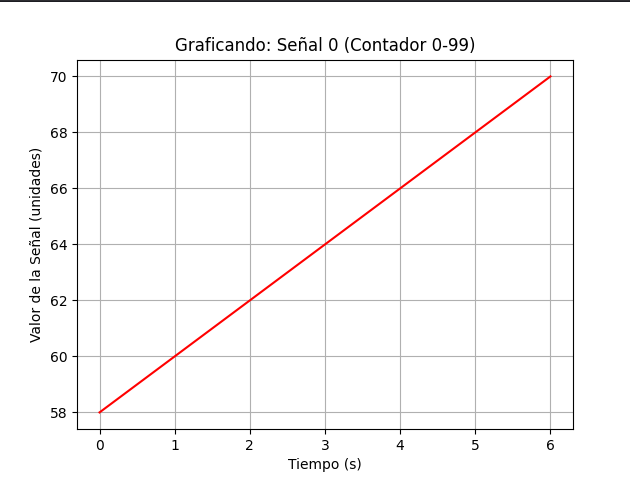
\includegraphics[width=0.8\textwidth]{img/graphic.png}
  \caption{Evolución de la Señal 0 (contador cíclico).}
  \label{fig:signal0}
\end{figure}

La Figura~\ref{fig:signal0} muestra cómo la Señal 0 avanza de 0 a 99 en pasos de 2 unidades por segundo. 

\begin{figure}[H]
  \centering
  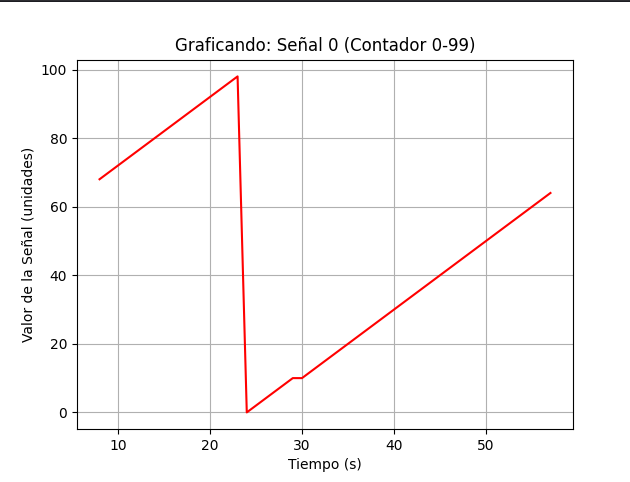
\includegraphics[width=0.8\textwidth]{img/graphic2.png}
  \caption{Forma de onda triangular de la Señal 1 (0–100).}
  \label{fig:signal1}
\end{figure}

La Figura~\ref{fig:signal1} ilustra la onda triangular de la Señal 1: sube linealmente de 0 a 100 y luego desciende de forma simétrica, con un periodo total de 2 segundos.

\FloatBarrier

\section{Conclusiones}

El presente trabajo práctico permitió recorrer desde los conceptos teóricos de la arquitectura \textbf{UEFI} hasta la implementación y prueba de un \emph{bootloader} propio, revelando la interacción detallada entre firmware, herramientas de \emph{toolchain} y hardware.

\begin{itemize}
  \item \textbf{UEFI como reemplazo de BIOS}. Comprendimos que UEFI no es una simple evolución sino una plataforma firmware escrita en~C, capaz de operar en 32~/ 64~bits, con servicios de arranque y ejecución en tiempo de \emph{runtime}, soporte GPT, \emph{Secure Boot} y controladores integrados. Aprender a invocar sus tablas (\texttt{BootServices} y \texttt{RuntimeServices}) habilita el desarrollo de utilidades de muy bajo nivel que conviven con el sistema operativo.
  \item \textbf{Superficie de ataque y riesgos}. Casos como \emph{LoJax}, \emph{ThinkPwn} o \emph{LogoFAIL} evidencian que vulnerar el firmware permite \emph{bootkits} persistentes aun tras reinstalar el SO. La seguridad del arranque exige tanto configuraciones correctas (protección de la flash) como la aplicación oportuna de parches.
  \item \textbf{CSME / ME y MEBx}. Las funciones de gestión remota (AMT) y arranque verificado (Boot Guard) ofrecen ventajas, pero el motor autónomo de Intel sigue siendo una \emph{caja negra} con fallos críticos publicados. Conocer MEBx resulta clave para equilibrar administración y exposición al riesgo.
  \item \textbf{coreboot: firmware libre}. coreboot demuestra que es posible reemplazar firmware propietario por una solución mínima y auditada, con arranques más veloces y menor superficie de ataque, manteniendo la flexibilidad gracias a los \emph{payloads} (SeaBIOS, TianoCore, LinuxBoot, etc.).
  \item \textbf{Herramientas de \emph{toolchain}}. Revisar el \texttt{linker} y la convención histórica de 0x7C00 mostró que los scripts de enlace son tan cruciales como el código; si el \emph{linker} desconoce la dirección final, los desplazamientos fallan y el arranque se aborta.
  \item \textbf{Bootloader ``HELLO''}. Desde ensamblar 512~bytes y firmarlos con \texttt{0xAA55}, hasta probar en QEMU y grabar en un pendrive, cerramos el ciclo completo: escribir, enlazar, testear y ejecutar código que arranca sin sistema operativo.
\end{itemize}

Además, el desafío final permitió poner en práctica conceptos clave de la transición al Modo Protegido:

\begin{itemize}
  \item \textbf{Transición Manual a Modo Protegido.} El diseño de un bootloader completamente manual, sin macros ni abstracciones, obligó a comprender en profundidad el flujo de activación del PE (Protection Enable), la importancia del salto largo posterior (\texttt{ljmp}), y la configuración explícita de los registros de segmento y la pila en 32 bits.
  \item \textbf{Uso Correcto de ELF y Linker Scripts.} La necesidad de ensamblar primero a ELF y luego enlazar usando un \texttt{link.ld} a 0x7C00 destacó el rol crítico del linker en sistemas bare-metal, resolviendo problemas típicos de formatos binarios directos (\texttt{-f bin}) como desincronizaciones y referencias incorrectas.
  \item \textbf{Segmentación y Protección.} Implementar descriptores diferenciados de código, datos R/W y datos R/O permitió experimentar directamente con la protección por hardware: definir un segmento de sólo lectura y verificar mediante ejecución que la CPU detecta y bloquea accesos inválidos.
  \item \textbf{Verificación de Protección por Hardware.} El intento de escribir en un segmento R/O, seguido de la observación de excepciones de Protección General (GP) y triple fallo en emuladores precisos como Bochs y QEMU-KVM, demostró empíricamente cómo el hardware asegura el cumplimiento de permisos segmentados, incluso antes de introducir mecanismos de paginación.
\end{itemize}

Estos ejercicios finales consolidaron no sólo la teoría del modelo de segmentación x86 y del proceso de arranque, sino también la práctica detallada de debugging en entornos reales (GDB, QEMU, Bochs), el entendimiento del rol de los selectores en modo protegido y la importancia de diseñar firmwares mínimos pero seguros.



\end{document}
